\documentclass[10pt,letterpaper]{article}
\usepackage{multicol}
\usepackage[utf8]{inputenc}
\usepackage{amsmath}
\usepackage{lipsum}
\usepackage{amsfonts}
\usepackage{amssymb}
\usepackage{graphicx}
\usepackage[margin=1in]{geometry}
\graphicspath{{../results/images/}}
\begin{document}
\begin{center}
\begin{huge}
Comparing the Parallel Scalability of Bucketsort, Samplesort, and Bitonic Mergesort to Serial Quicksort\\
\end{huge}
\vspace{0.25in}
\begin{large}
Coen Valk, Bradford Stone\\
valkc@rpi.edu, stoneb2@rpi.edu\\
\end{large}
\end{center}
\vspace{0.25in}
\begin{multicols}{2}
\begin{abstract}
One of the most primitive and vital operations possible on arrays is sorting. Not only is sorting important for data organization, it is a prerequisite for many more complex array operations. Therefore, it is vital that any sorting algorithm used often is extremely efficient, and able to use available resources as well as possible. In this paper, we test the strong scalability of three different parallel sorting algorithms on an IBM Blue Gene Q system. Furthermore, we test the performance of each algorithm as the size of the array increases and present results for the quickest algorithm in each situation.
\end{abstract}
\section{Introduction}
As the size of input arrays into a sorting algorithm grows, as does the execution time. In serial sorting algorithms, only one comparison is made at a time, while the rest of the array sits idle. Parallel sorting algorithms unlock a new potential to compare multiple parts of the array at the same time, then merging the results to create a full sorted array. High performance computing gives users the ability to greatly speedup execution time by parallelizing the sorting algorithm.

Both members of this project worked together to implement the three sorting algorithms, run the algorithms on the Blue Gene Q system and compile all results. Coen Valk implemented the bitonci mergesort and samplesort, while Brad implemented the bucketsort. Both members wrote about the analysis of the algorithms they implemented in the paper.

\section{Background}

Since sorting is such a essential array operation, ever since the beginning of parallel computation, there has been research to further push the boundaries of sorting algorithm efficiency. Many papers have provided new insight to improving the execution time of sorting large arrays. In particular, one paper which proposes an in-place super scalar samplesort (IPS$^4$o) is rather interesting and a novel proposal building upon an already effective sorting algorithm super scalar samplesort (s$^3$).

IPS$^4$o builds upon the groundwork set by the implementation of $s^3$ \cite{10.1007/978-3-540-30140-0_69} and adds a few key details that make it an extremely effective sorting algorithm proposal \cite{DBLP:journals/corr/AxtmannWF017}. Making effective use of threads and shared memory, each thread is treated as a bucket in the samplesort. IPS$^4$o is different from s$^3$ in how the steps are completed in order to keep IPS$^4$o in-place as well as give the opportunity for parallel sorting. In particular, all of the four steps, except for the first sampling step, are slightly different in IPS$^4$o compared to s$^3$. The second step of samplesort, local classification in IPS$^4$o combines all adjacent elements into larger blocks, each element of which are all members of the same bucket. This is done in place, requiring only a small buffer to contain blocks that are not ready to be added back to the input array as a complete block yet. The third step, Block permutation places blocks in the correct order throughout the input array. This puts all of the elements in approximately the right order, but still requires the final cleanup step to ensure that elements around the boundaries of blocks and threads are in the correct position. This four step process can be parallelized by having each thread perform the same action on a smaller part of the array, and switching blocks with each other during the block permutation phase.

IPS$^4$o proves itself to be an excellent choice as a sorting algorithm, ensuring average case $O(n \log n)$ with a high probability, very low branch mispredictions similar to $s^3$, and improves upon $s^3$ by being in-place and higher potential for parallelization. This samplesort implementation also outperforms many similar comparison based sorting algorithms in serial as well as parallel conditions and many different architectures, as shown by the paper.

The largest difference between our implementation and IPS$^4$o is our use of distinct processes and MPI ranks instead of shared memory and threads, and is therefore not in-place. Because of the lack of shared memory, our implementation will most likely suffer when it comes to rank communication and sending blocks to the other buckets.

Another paper that highlights the differences in efficiency is Pasetto and Ahkriev's comparison on parallel sorting algorithms \cite{Pasetto:2011:CSP:2048147.2048207}. Their analysis is limited, but their results concisely summarize the parallel performance of 6 sorting algorithms on two different CPU architectures. This paper does reference synchronization as a key factor in slowing down the sorting algorithm with larger processes, or when arrays are small (under 100 thousand elements or so). In these smaller cases, serial sorting algorithms were even preferred over the other parallel sorting algorithms analyzed in the paper.

\section{Analysis}
\subsection{Setup}
Each sorting algorithm was implemented to sort an array of integers given to the root rank. Each array is initialized as a list of random positive integers. The experiment was repeated with array sizes from $2^{20}$ elements up to $2^{25}$ elements, with all powers of two in between tested as well. For each array size, each sorting algorithm was run in parallel from 2 ranks up to 4096 ranks. Each experiment was run on the RPI Blue Gene Q high performance computer. The wall clock execution time for each run was recorded, and the results were compiled to show the strong scaling properties of each algorithm. The results of the scalability of each algorithm is compared with a serial quicksort to show the speedup of parallel sorting algorithms.
\subsection{Serial Quicksort}
A quicksort implementation was used as a good quality serial sorting algorithm to create a baseline for the relative speedup of parallelizing sorting in a high performance computing environment. Quicksort is often referred to as one of the fastest serial sorting algorithms for an array of randomly distributed numbers \cite{10.1093/comjnl/5.1.10}. In this context we will show that certain parallel sorting algorithms in the right conditions will consistently outperform quicksort in a sorting task.

It is important to note that quicksort only performs optimally on mostly randomly organized graphs, as quicksort depends heavily on choosing the proper pivot to split the array in half \cite{10.1093/comjnl/5.1.10}. In worst-case conditions, such as a nearly sorted graph, quicksort can have up to a $O(n^2)$ runtime. If in future work other distributions of numbers are chosen, other sorting algorithms such as mergesort may need to be the new baseline to show serial sorting performance \cite{Knuth:1998:ACP:280635}.

The quicksort implementation is from the C \texttt{stdlib.h} library. This implementation will be used as a baseline to see the advantages of parallel speedup when sorting.
\subsection{Bucketsort}
The most interesting attribute of bucketsort is that elements are not pairwise compared. Instead, based on certain attributes they are separated into buckets. In this example, each bucket is an MPI rank. The root sends elements to the proper mpi rank bucket based on the remainder when divided by the number of ranks. then the results are all gathered. The process repeats, putting elements in buckets based on the next series of bits. Eventually this will lead to a sorted sequence of numbers.

With randomly distributed arrays of integers, bucketsort can effectively organize large arrays quickly. However, with many duplicate numbers, or gaussian distributions with a small standard deviation, certain buckets may be much larger than others causing imbalanced load between processes. Imbalance in workload per process may cause significant slowdown due to available resources not being effectively used.

Bucketsort of course depends on the number of elements, but also depends on the size of the largest element to be sorted. The largest element in the array determines how many iterations of bucket sorting 
\subsection{Samplesort}
Samplesort is an effective sorting algorithm, similar to bucketsort, where each element is fit into buckets based on it relative size in the array. Different from bucketsort, however, is the clever choosing of pivots from a samples of the array to better balance load between all processes
\cite{samplesort}. Samplesort splits the array into equal parts given to each MPI Rank. Each MPI Rank serially sorts the smaller array. From the sorted arrays, regularly spaced out samples are gathered to the root and merged to make an array of samples. The root selects n pivots, where n is the number of MPI ranks, regularly spaced out from the sample array. This information is scattered to each rank. Following this, each rank determines which other rank to send data to, based on the pivots. Each rank gathers data using \texttt{MPI\_Gatherv} from all other ranks which fit within its pivot window. Gathering all results from each rank takes some time, so at a certain point the time taken to communicate between ranks for gathering elements will actually begin to increase the runtime once again.

Because samplesort takes care to pick samples that will balance workload evenly across ranks, Samplesort will most likely show a consistent runtime for different distributions of elements as well such as almost sorted, completely backwards, or Gaussian distribution.

Due to time constraints, our implementation of samplesort only works properly when the number of elements is a multiple of the number of MPI ranks. This is not a requirement of samplesort, but does make implementation for the last bucket easier. This is also taken into account in the experiments, as the number of elements as well as the number of ranks are both powers of two.
\subsection{Bitonic Mergesort}
Bitonic mergesort, otherwise known as batcher sort or odd-even mergesort takes advantage of bitonic sequences to sort an array of numbers \cite{Knuth:1998:ACP:280635}. Bitonic arrays contain only one local maximum and one local minimum. Bitonic mergesort merges multiple bitonic sequences into one larger bitonic list, until the entire list can be merged in ascending order. Serially, bitonic mergesort is not as efficient as it could be, due to the constant shuffling and reshuffling into different sized bitonic sequences. However, when executed in parallel, every rank can contribute to creating a bitonic sequence. Therefore, there will most likely be a significant speedup when set in parallel compared to a serial version of bitonic sort. Below is a diagram depicting the comparisons required for bitonic mergesort. For each iteration, all of these comparisons can be completed in parallel, so there is much potential for parallel speedup.

\begin{center}
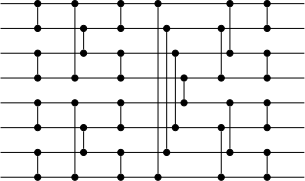
\includegraphics[scale=0.7]{bitonic_diagram}
\end{center}

One particular quirk of Bitonic Mergesort is that the size of the array must be a power of two, due to the process of merging bitonic sequences. This was accounted for in this experiment by making all of the tested array sizes a power of two, but it is possible that this may restrict use for this sorting algorithm in the real world. In order to sort an array of size $n$ that is not a power of two, a new array would need to grow to the next power of two above $n$, and initialize the rest of the elements as an "infinity" value so that the array will be sorted, with the fake "infinity" values still at the end of the array. In the real world, this is extremely inefficient, as there may be situations in which the array is nearly twice as large as it needs to be to sort every number, which may waste memory resources as well as increase wall clock execution time.
\section{Resuts}
After all of the results are compiled, a graph depicting the scalability of each sorting algorithm was created. Bucketsort, while the wall clock time is slower than the other two algorithms, showed significant speedup as the number of available processes increases. The following graph shows the execution time of sorting all of the numbers with our bucketsort implementation as the number of processes varies. In this example, some of the experiments did not even complete within the 30 minute requirement. In particular, the 2 rank experiment sorting $2^{24}$ elements and the 2 and 4 rank experiments sorting $2^{25}$ elements. Furthermore, this implementation of bucketsort seemed to be less consistent compared to the consistency in scalability of bitonic mergesort and samplesort. In the graph below, each curve represents a different number of elements in the array which needs to be sorted:

\begin{center}
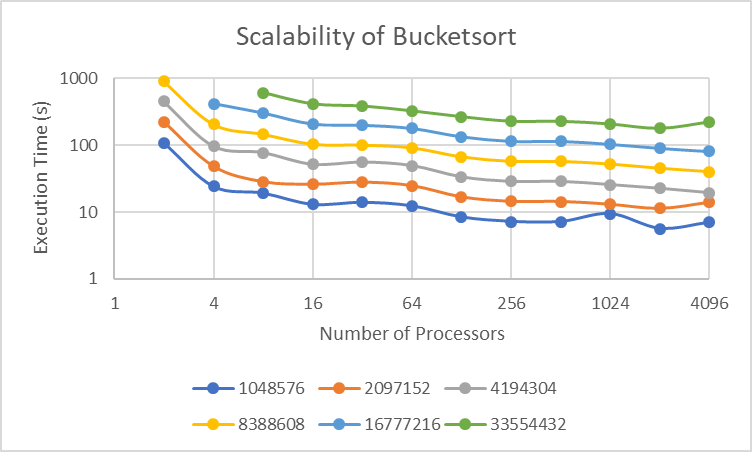
\includegraphics[scale=1.3]{bucket_scale}
\end{center}

Unfortunately, our implementation of bucketsort, while it scaled well with itself, did not show promising results when compared with the serial quicksort implementation. In fact, this bucketsort implementation showed a consistent speed-down compared to quicksort. Future work could investigate other ways to implement bucketsort which may decrease execution time.

\begin{center}
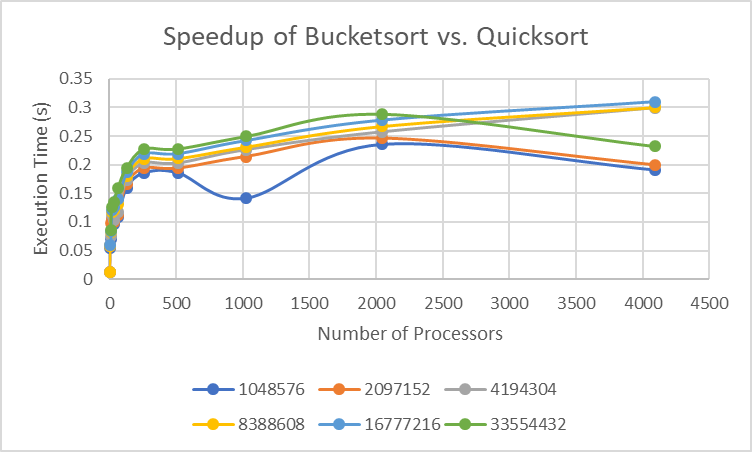
\includegraphics[scale=1.3]{bucket_speedup}
\end{center}

Bitonic mergesort on the other hand shows particularly impressive scalability. At the largest number of elements, bitonic sort was clearly the fastest algorithm, with an execution time of less than half a second to sort $2^{25}$ elements. Validating our suspicions, at a low number of processors, bitonic sort performs slower than samplesort, but quickly catches up and improves upon samplesort's scalability as the number of processes increases. The following graph demonstrates the execution time of sorting $2^{25}$ elements based on the number of processors.

\begin{center}
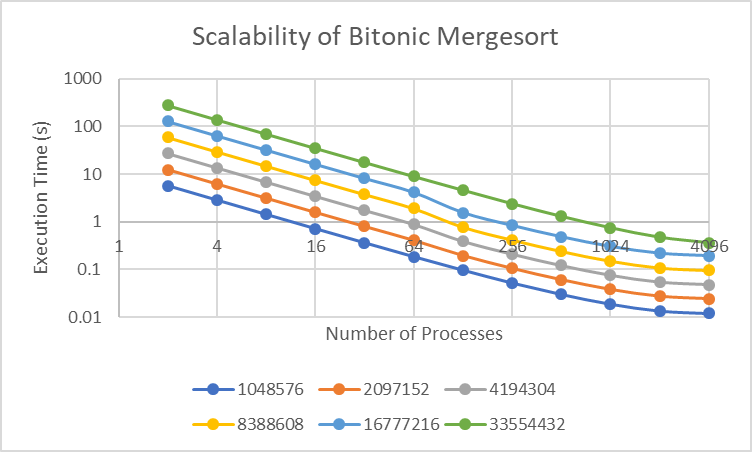
\includegraphics[scale=1.3]{bitonic_scale}
\end{center}

This result is extremely desirable, and the effect of parallelizing bitonic mergesort is clearly visible in the following graph. This graph shows up to 140 times speedup in ideal circomstances from a serial quicksort implementation.

\begin{center}
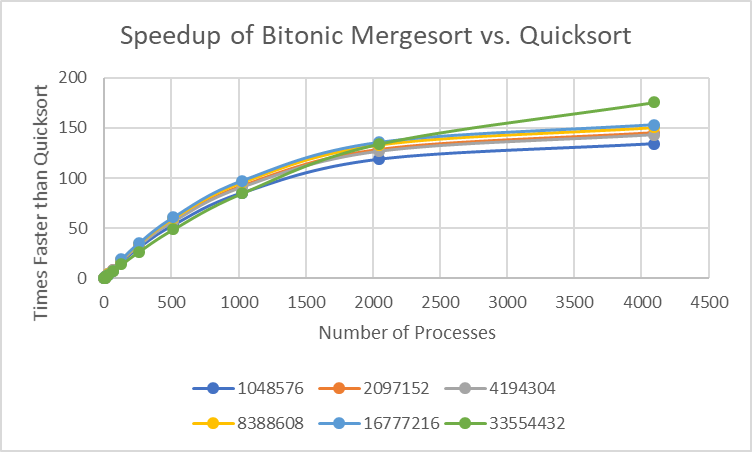
\includegraphics[scale=1.3]{bitonic_speedup}
\end{center}

Samplesort also showed speedup - to a certain extent - as the number of processes increased. It seems that there exists a happy medium between having a small enough array, but not too small to small to send too many messages across ranks. The ideal point seems to be at either 32 or 64 ranks. Beyond that number of ranks, communication between ranks slows down the execution time of the program. Under these number of ranks, the size of each array is large enough that traversal of the local array causes slowdown of the algorithm.

\begin{center}
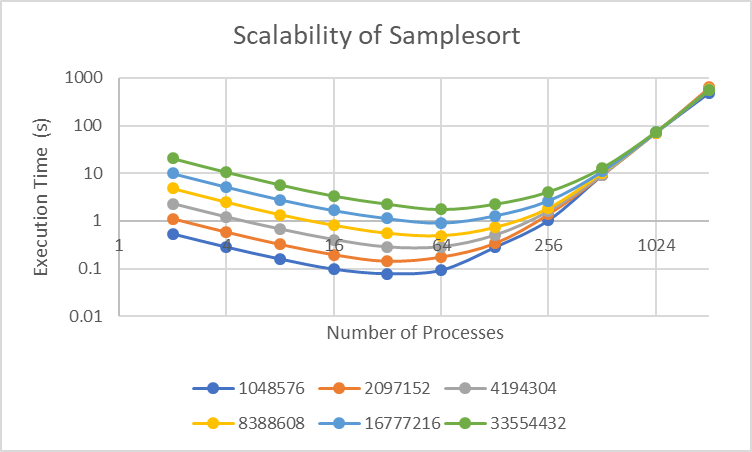
\includegraphics[scale=1.3]{sample_scale}
\end{center}

The following speedup graph shows how samplesort beings slower than quicksort, at 32 or 64 ranks reaches a peak efficiency, then quickly drops off again, eventualy to be slower than quicksort once again. At this ideal point however, there is a convincing up to 35 times speedup compared to a serial sorting algorithm.

\begin{center}
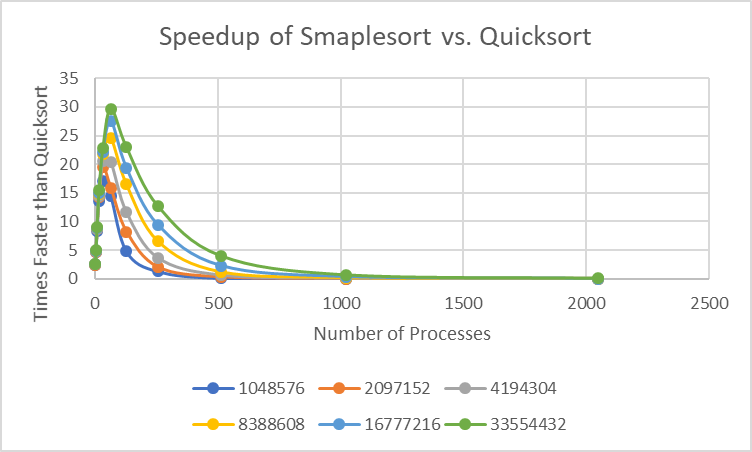
\includegraphics[scale=1.3]{sample_speedup}
\end{center}

However, what is most interesting about samplesort is how the algorithm scales with the number of elements. With a large number of processors, the execution time is quite large, but increases only slightly, compared to the doubling of the number of elements being sorted. Typically execution time at least doubles when the number of elements doubles. The following graphs depict the small increases in execution time of samplesort at 512 and 2048 processors and varying number of elements.

\begin{center}
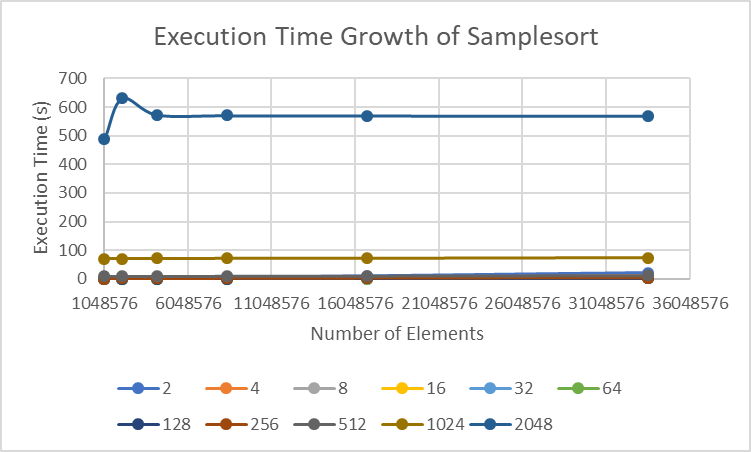
\includegraphics[scale=1.3]{sample_growth}
\end{center}

This is very different from the scalability of the other two algorithms as shown below. As the number of elements increases, the execution time increases similar to the theoretical limit asymptotic runtime of $O(n \log n)$.

\begin{center}
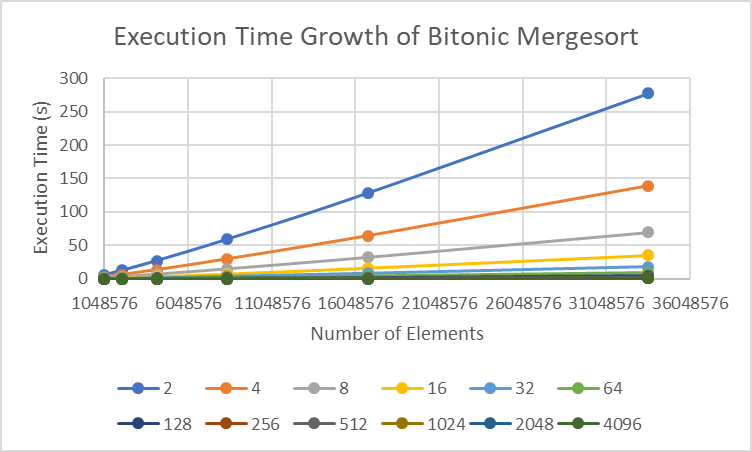
\includegraphics[scale=1.3]{bitonic_growth}
\end{center}

The growth in execution time as the number of elements to be sorted increases in bitonic mergesort is much steeper than the curve seen in the samplesort graph. A very similar trend to bitonic mergesort and quicksort can be seen in bucketsort as well, despite its relative slowness compared to the other sorting algorithms analyzed.

\begin{center}
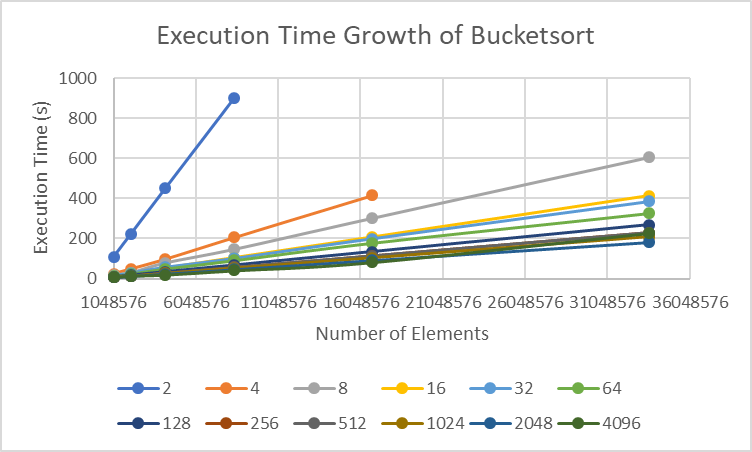
\includegraphics[scale=1.3]{bucket_growth}
\end{center}

The growth of both the bitonic mergesort and the bucketsort curves are more consistent with the growth in execution time of the serial quicksort implementation as number of elements in an array increases, as seen below. More analysis would need to be done to explain why the samplesort growth curve does not fit the other sorting algorithms' growth curves.

\begin{center}
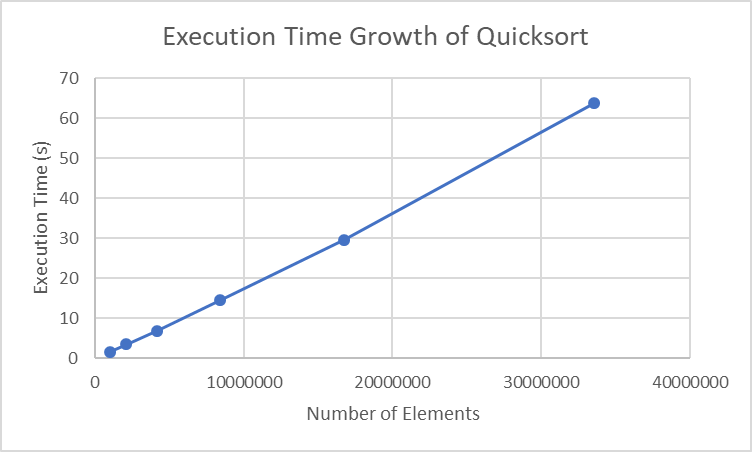
\includegraphics[scale=1.2]{quick}
\end{center}

\section{Conclusion}
There is research here that can expand on in further analysis. As mentioned earlier, the current experiment only analyses performance of a list of randomly ordered integers. However, depending on the distribution or ordering of the elements in an array performance can be quite different. Future work could include analysis of the same algorithms with a nearly sorted list, a backwards sorted list, a Gaussian distribution, or a large number of repetitive elements. All of these environments could affect the runtime of each algorithm, and knowing more about the distribution of the input array may affect decisions about the ideal sorting algorithm to use.

Another opportunity for growth in this project may be to combine sorting algorithms together, based on their strengths, to create an effective and even more scalable large array sorting method. Depending on the situation, the program could determine a good quality sorting algorithm to use in that case, instead of using one sorting algorithm as a catch-all solution for all arrays. Another area to expand upon is how using threads to further increase parallelism as well as take advantage of shared memory to speed up sorting algorithms. In small core cases, using threads has been shown to speed up the execution time of parallel sorting algorithms \cite{DBLP:journals/corr/abs-1808-10292}. Taking advantage of threads may also help to make a more scalable sorting algorithm.

One note to consider about parallel sorting algorithms is how often they require large amounts of memory outside of the original array. Serial quicksort works completely in-place, while the parallel sorting algorithms analyzed all use much more memory than just the original input array. Great care must be taken to decide whether the added memory usage is worth the speedup in execution time. In high performance computing, with extremely large problems but plenty of sufficient resources, it may be reasonable to prefer a lower execution time over lower memory usage.

Overall, as is visible from the data, it is evident that parallel bitonic mergesort is an excellent choice when there are very many ranks available that can be devoted to sorting. This could potentially result in a 140 times speedup in sorting large arrays. However, bitonic sort wastes many resources when the array to be sorted is not a power of two. When fewer ranks are available or when the number of elements is not a power of two, Samplesort is a good option for sorting a very large number of elements. Samplesort results show that it is most effective when used with between 32 and 64 ranks, resulting in up to 30 times speed up compared to a serial quicksort. Bucketsort shows promising scalability, but this implementation is much slower than the other sorts analyzed. Overall, parallel sorting algorithms are an important contribution to any high performance computing system, enabling users to quickly and efficiently sort very large arrays of numbers with available resources.

\bibliographystyle{acm}
\bibliography{bibliography}
\end{multicols}
\end{document}